%
% Use the standard article template.
%
\documentclass{article}

% The geometry package allows for easy page formatting.
\usepackage{geometry}
\usepackage{float}
\geometry{letterpaper}


% Load up special logo commands.
\usepackage{doc}

% Package for formatting URLs.
\usepackage{url}

% Packages and definitions for graphics files.
\usepackage{graphicx}
\usepackage{epstopdf}
\DeclareGraphicsRule{.tif}{png}{.png}{`convert #1 `dirname #1`/`basename #1 .tif`.png}

%
% Set the title, author, and date.
%
\title{Skeuomorphic Design}
\author{Eric Dea}
\date{October 30, 2012}


%
% The document proper.
%
\begin{document}

% Add the title section.
\maketitle

% Add an abstract.
\abstract{
This paper explains how skeuomorphic interface designs fit the user's and developer's mental model.  Skeuomorphic designs are intended to create a familiar layout for users, especially new or novice users.  Effectively aligning user and developer mental models is exactly what skeuomorphism is about. When trying to create an effective usable interface, skeuomorphism comes to the mind of the developer.  This paper will show that the usability of skeuomorphic user interface designs is directly related to the successful alignment of the user and developer mental models.}

% Add various lists on new pages.
\pagebreak
\tableofcontents

\pagebreak
\listoffigures

\pagebreak
\listoftables

% Start the paper on a new page.
\pagebreak

%
% Body text.
%
\section{Introduction}
\label{introduction}

A Skeuomorph, or Skeuomorphism, is when a product imitates design elements functionally necessary in the original product design, but that becomes ornamental in the new product design \cite{wiki}.  So in the computer world, a skeuomorphic user interface design is one that tries to imitate a 'real world' interface by using various decorations.  The website interface designer tries to replicate what the user's mental model is, what the user pictures in their mind.  This relationship between the user's mental model and the developer's mental model is key to creating a successful user interface.  In this paper, I hope to show how important this relationship is and how skeuomorphism directly relates to this relationship between the user and developer's mental models.


\section{Skeuomorphism}

In a User Interface, the elements of the interface can either be functional or non-functional.  The functional elements can either be skeuomorphs or just plain old elements that are necessary to the interface.  The non-functional elements are there for decoration and visual satisfaction.  This is where skeuomorphs come into play, for they create a better looking layout for most novice computer users.

\subsection{Non-Functional Elements}

Skeuomorphism, or skeuomorphs, have a certain abstract quality and property.  The layout and content of a user interface must have components that can be made abstract, or nonfunctional.  An abstract component can serve both as a building block for new development and as a reminder of its future functionality \cite{skeu-software}. So, even though most of these 'abstract' elements are non-functional and are just decorations, there is an option for future development to make these elements functional.  An example of this abstract element, or non-functional, is the rip/tear on Apple's iCal.

\begin{figure}[H]
\centering
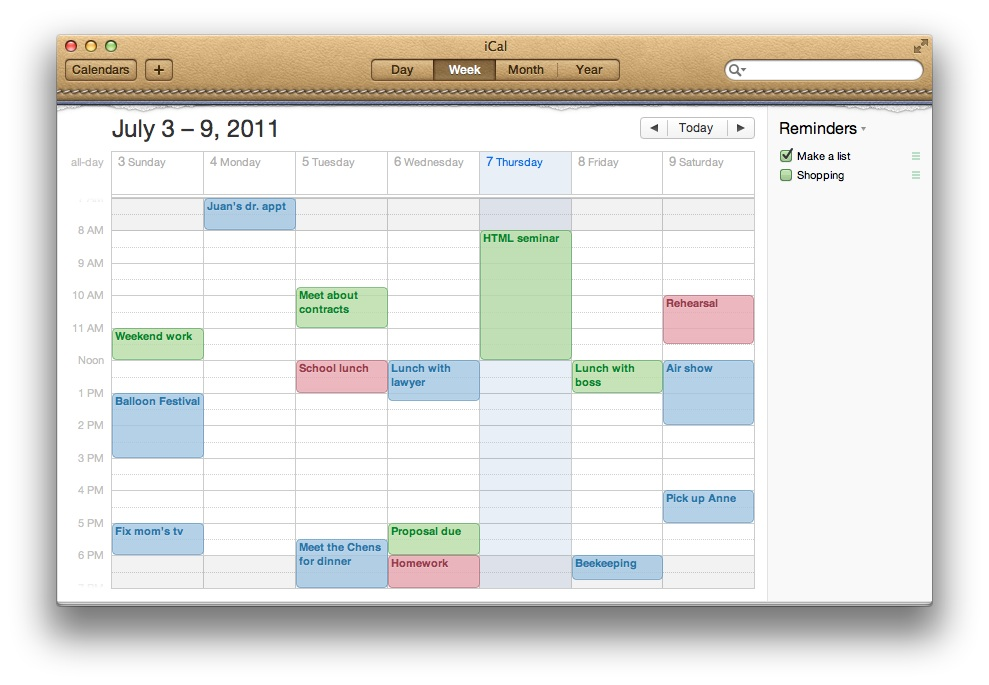
\includegraphics[width=3.5in]{ical.jpeg} 

\caption{iCal with Skeuomorphism}
\label{iCal}
\end{figure}

If you look at the top of Figure \ref{iCal}, there are rip marks indicating that the user 'ripped' out the past month, just like an ordinary calendar.  The tear has no functionality, for it is just there for decoration.

\subsection{Functional Elements}

On the other side of Skeuomorphism, there are elements of a user interface that exactly replicate the real life version and also have functionality.  One common example of this is Figure \ref{traktor}, which is a DJ mixing software Traktor.

\begin{figure}[H]
\centering
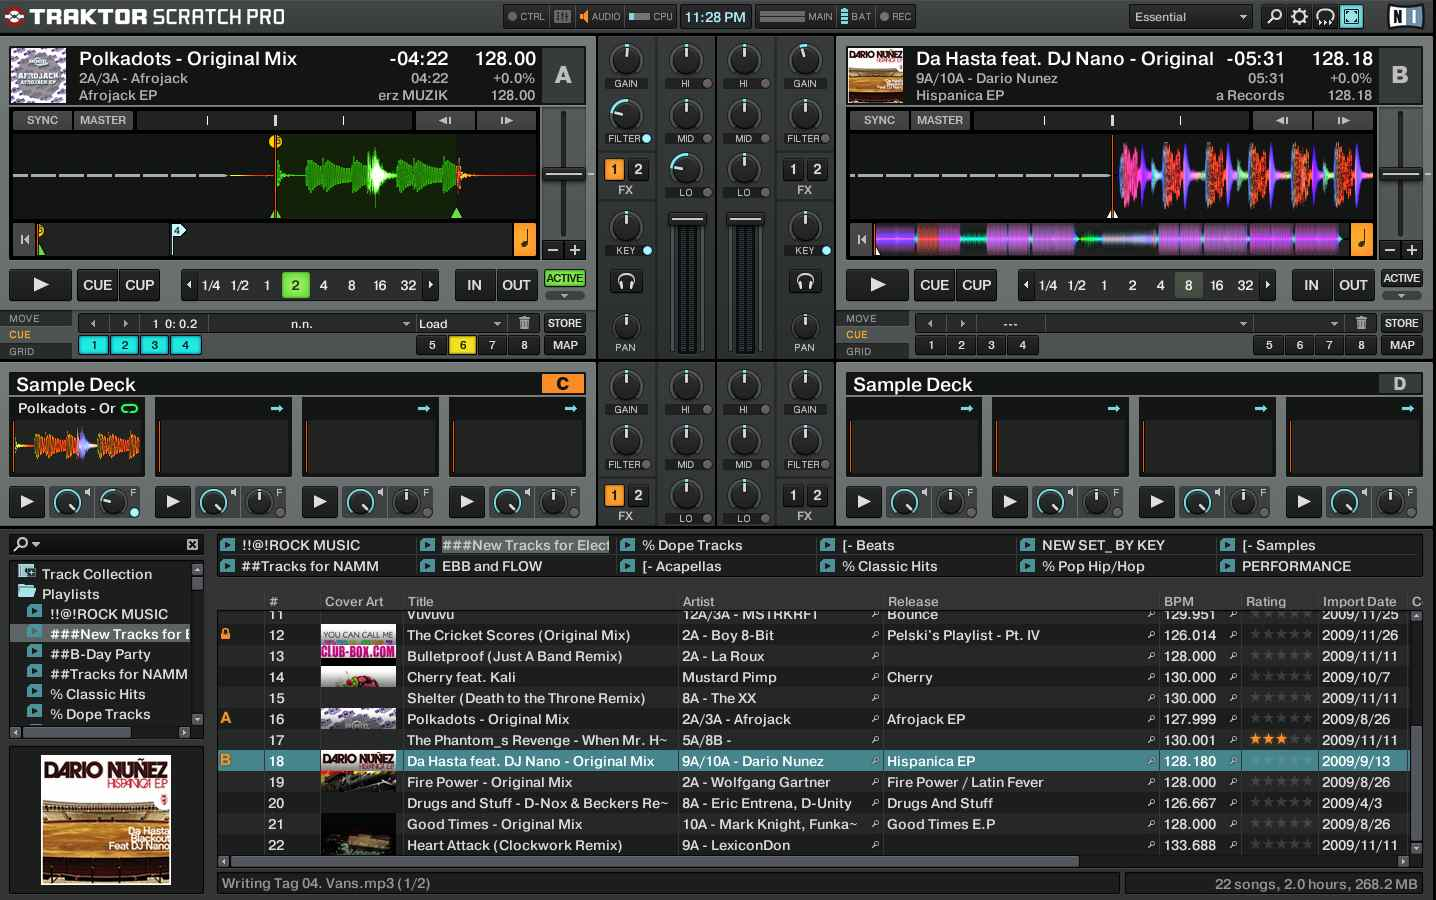
\includegraphics[width=4.5in]{traktorUI.jpg} 

\caption{Traktor Scratch Pro 2}
\label{traktor}
\end{figure}

All of the buttons and knobs on the interface are fully functional.  A DJ mixing set has very similar, if not exact, buttons and knobs.  Because all of the knobs are turned just like a real DJ mixer, the skeuomorphic elements are functional.  A skeuomorphic user interface where all of its elements are functional is the perfect interface where the user's mental model and the developer's mental model is on the same page.  For example, say the user is a DJ who uses mixers but has not ever DJed on a computer.  If this user were to try out this digital interface, the transition is very easy for everything on his own mixer looks and works exactly the same on the computer.

\section{Mental Model}

A mental model is an explanation of someone's thought process about how something works in the real world \cite{wiki-mental}.  When trying to successfully align the mental models of the user and the developer, their thought processes must be similar.  Because skeuomorphism is the imatating of elements to a new product, the quality of the skeuomorphism is directly related to the developer's alignment of the mental model of the user.


\subsection{Multiple Outline Levels}

\LaTeX\ has support for up to three outline levels (\verb!\section!, \verb!\subsection!, and \verb!\subsubsection!).  It also recognizes \verb!\paragraph! and \verb!\subparagraph! directives, though those don't show up in the table of contents.  All of these directives expect a title.

Note also the use of the \verb!\verb! directive for inserting code-like labels or symbols.  It was particularly needed here so that we can include the backslash character in the text.

\subsection{Tables and Figures}

\LaTeX\ has full support for tables and figures.  Table~\ref{table-sample} shows a sample table and Figure~\ref{figure-sample} shows a sample figure.  Note the built-in support for captions and the automated numbering functionality.  Lists of tables and figures can also be automatically generated, as seen at the beginning of this document.




One very important thing to remember about how \LaTeX\ handles tables and figures by default: you don't have to worry about where they go exactly.  The general rule is that you insert them in the source after your first reference to them, and \LaTeX\ determines their final position.  It also makes decisions on how much page space to devote to them.  This all follows \LaTeX's overall theme of focusing on the content of your paper, and not its format.

Just so you can see a second table, Table~\ref{table-sample2} is provided.


\section{Another Section}

We're adding another section just so you can see how that looks.  Plus there are a few more \LaTeX\ features to illustrate.

\subsection{Bulleted and Numbered Lists}

\LaTeX\ is very good at providing clean lists.  Examples are shown below.

\begin{itemize}
\item Bulleted items come out properly indented and spaced, every time.

\begin{itemize}
\item Sub-bullets are a virtual no-brainer: just nest another \verb!itemize! block.
\item Note how the bullet character automatically changes too.
\end{itemize}

\item Just keep on adding \verb!\item!s\ldots

\item \ldots until you're done.
\end{itemize}

Numbered lists are almost identical, except that you specify \verb!enumerate! instead of \verb!itemize!.  List items are specified in exactly the same way (thus making it easy to change list types).

\begin{enumerate}
\item A list item
\item Another list item
\item A list item with multiple nested lists

\begin{itemize}
\item Nested lists can be of mixed types.
\item That's a lot of power and flexibility for the price of learning a handful of directives.

\begin{enumerate}
\item Like nested bullet lists, nested numbered lists also ``intelligently'' change their numbering schemes.
\item Meanwhile, all \emph{you} have to write is \verb!\item!.  \LaTeX\ does the rest.
\end{enumerate}
\end{itemize}

\item Back to your regularly scheduled list item

\end{enumerate}

\subsection{Subsection with Another Figure}

We may as well include a second figure also, shown in Figure~\ref{figure-sample2}.  The same image file is used, but note how it can be resized.  Again, observe how the positions of the tables and figures do not necessarily match their positions in the source file, reiterating the aforementioned \LaTeX\ functionality for deciding where these items go in the final document.  You provide an approximate location, and \LaTeX\ does the rest.

\begin{figure}
\centering


\caption{Another sample figure}
\label{figure-sample2}
\end{figure}

\section{Conclusion}

Wrap up your paper with an ``executive summary'' of the paper itself, reiterating its subject and its major points.  If you want examples, just look at the conclusions from the literature.

% Generate the bibliography.
\bibliography{cmsi370-skeuomorphic}
\bibliographystyle{unsrt}

\end{document}
